\graphicspath{{07-PID/Figures/}}

\section{Particle ID}
\label{Sect:PID}

While the protons in the MICE beam can be effectively removed before entering the detectors~\cite{proton_absorber}, the remaining particles are a mix of pions, muons, and electrons.  Effective particle ID (PID) methods are required to ensure that we are measuring the cooling of muons rather than of other particle species.  While earlier studies in MICE were performed with a beam optimized for muon purity~\cite{2016JInst..11P3001A}, accurate particle ID algorithms allow us to optimize for muon yield rather than purity.

{\color{red}Work is ongoing on an alternate multivariate likelihood-based PID algorithm, but the currently-used cut-based algorithm will be described here.}

\subsection{Algorithm}
\label{SubSect:PID_Algo}

The PID algorithm uses the TOF and Tracker detectors.  TOF0 and TOF1 can be combined with the upstream tracker to ID a particle upstream of the absorber.  However, if the particle has decayed while travelling through the detector, a downstream identification is more difficult due to the fact that there is no entirely-downstream TOF measurement.  TOF1 and TOF2 can be combined with the downstream tracker, but the uncertainty in the PID is increased due to the particles' energy loss in the absorber.

A particle's momentum can be calculated by the curvature of its track in the tracker's solenoid field, while its velocity can be calculated from the time-of-flight and the path length.  From these, the particle's mass can be calculated:

\begin{equation}
\label{eq:pid_mass_calc} m = {p \sqrt{1-(v/c)^2} \over v/c}
\end{equation}

the particle can then be determined to be a pion ($m=140$ MeV), muon ($m=105$ MeV) or electron ($m=511$ keV).

This method requires an accurate measurement of the particle's path length between the TOF detectors, which will be slightly longer than the straight-line distance between the detectors due to the magnetic fields involved.  The time-of-flight of electrons is used to calibrate this distance, since electrons are moving very close to the speed of light ($\gamma \approx 500$) at these beam momenta.  Therefore, after a fit of the electron TOF peak in a particular beam setting, each particle's $v/c$ is calculated as $\mathrm{TOF}_e / \mathrm{TOF}$.

Additionally, this calculation assumes that the measurements of TOF and momentum were performed at the same point.  Since the particle has lost momentum between the TOF and Tracker detectors, a correction must be added.  Figure~\ref{fig:tof_track}(a) shows that before this correction, the data points are well-separated into different particle species, but are slightly displaced from their naively-expected positions.

To find this correction, a loose cut is performed on the data to find particles that are near the muon mass.  A fit is performed on these particles to find a momentum offset to be applied in Equation~\ref{eq:pid_mass_calc} to ensure that the muons are centred at the muon mass of $105.7$ MeV.  Figure~\ref{fig:tof_track}(b) shows the same data as in (a), but the expected pion and muon curves have been adjusted with this momentum offset.

After the above parameters $\mathrm{TOF}_e$ and $p_\mathrm{offset}$ have been found, the PID algorithm can be applied to each track to calculate a mass for the particle, as shown in Figure~\ref{fig:pid_mass}.  Analyses may require different cuts on this variable due to different purity requirements, but pions and muons are sufficiently well-separated to allow good identification.

\begin{figure}
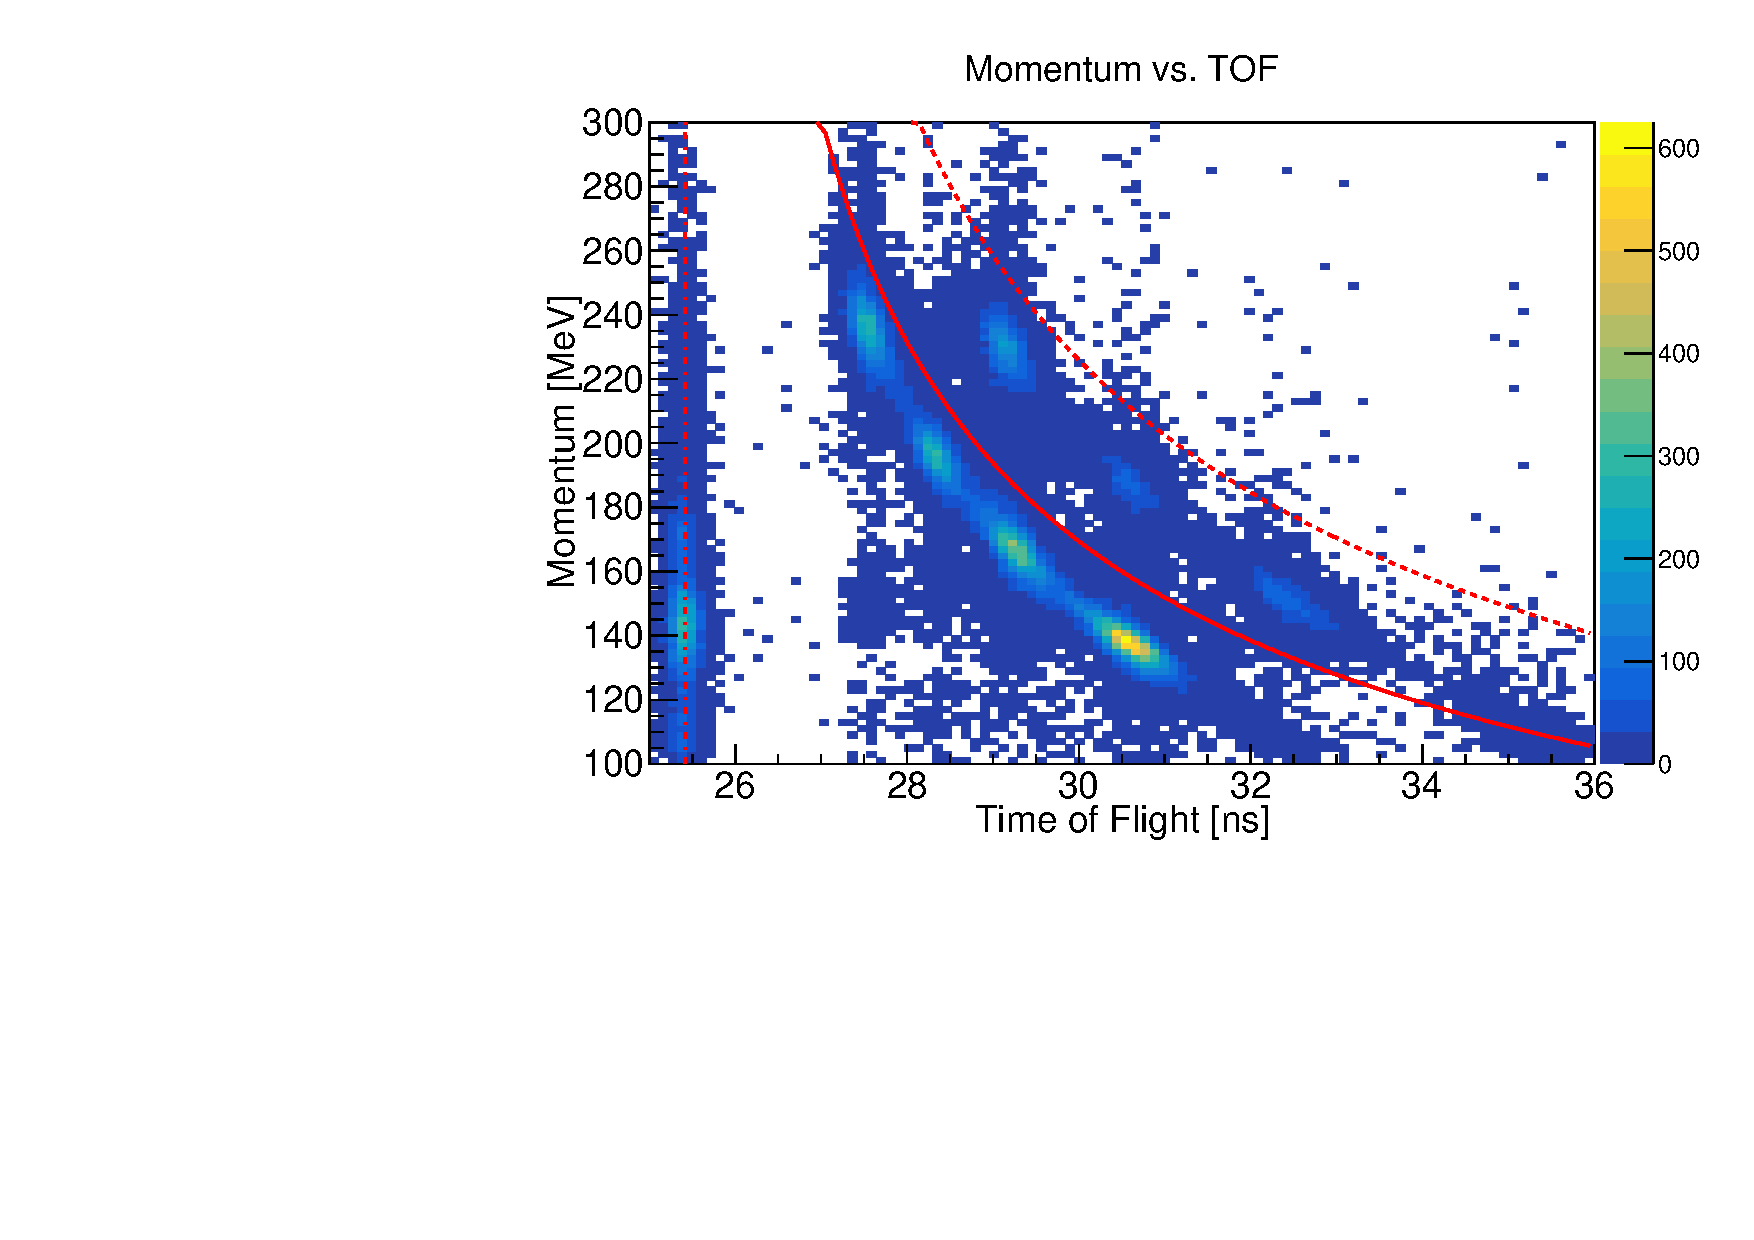
\includegraphics[width=0.45\textwidth]{uncorrected_track_tof.pdf}\hfil
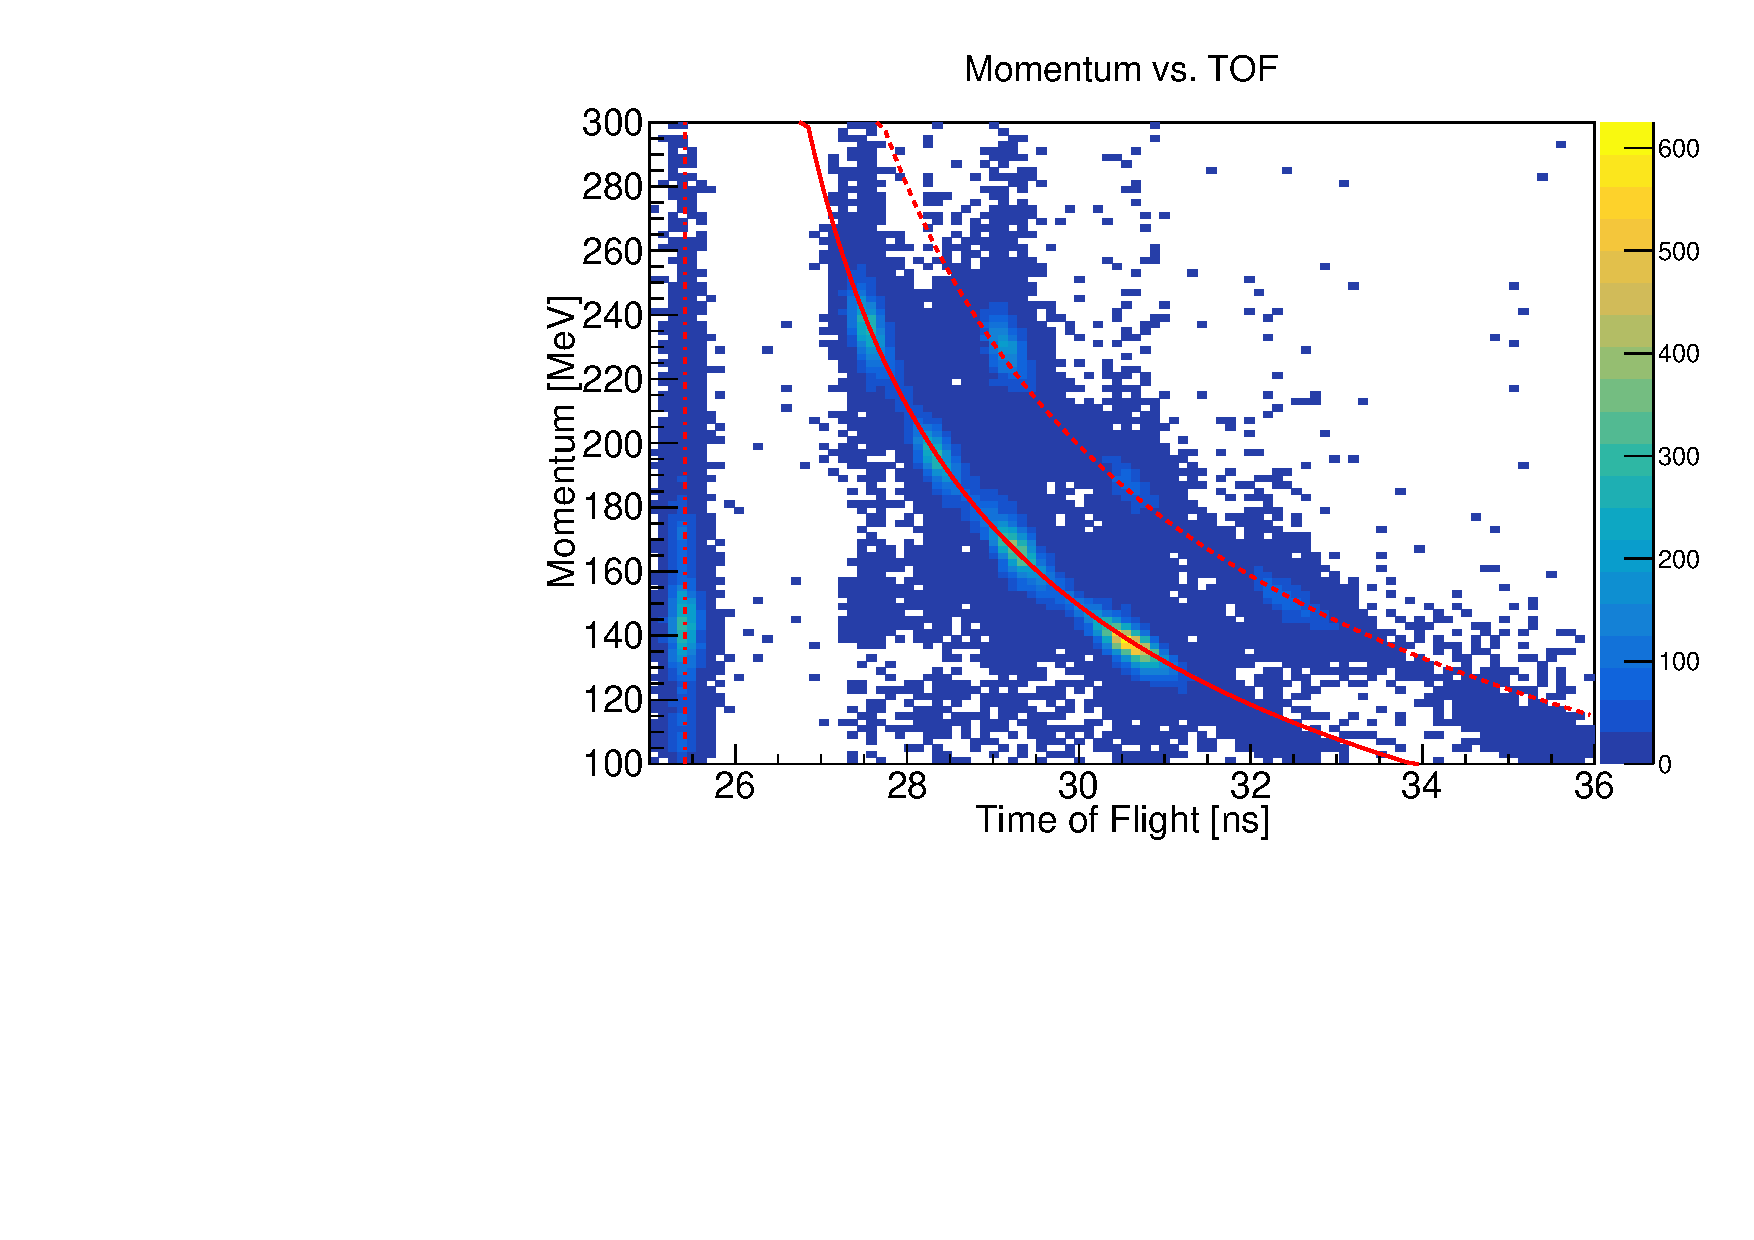
\includegraphics[width=0.45\textwidth]{corrected_track_tof.pdf}
\caption{The TOF measurement and Tracker momentum of particles in a selection of MICE runs with different momentum settings for the beam.  The solid lines show the expected momentum vs. TOF for pions at $m=140$ MeV, muons at $m=105$ MeV) and electrons at $m=511$ keV.  (a) shows this expected relation assuming no energy loss between TOF and Tracker detectors.  (b) shows the expected relation after correcting for this energy loss.}
\label{fig:tof_track}
\end{figure}

\begin{figure}
{\centering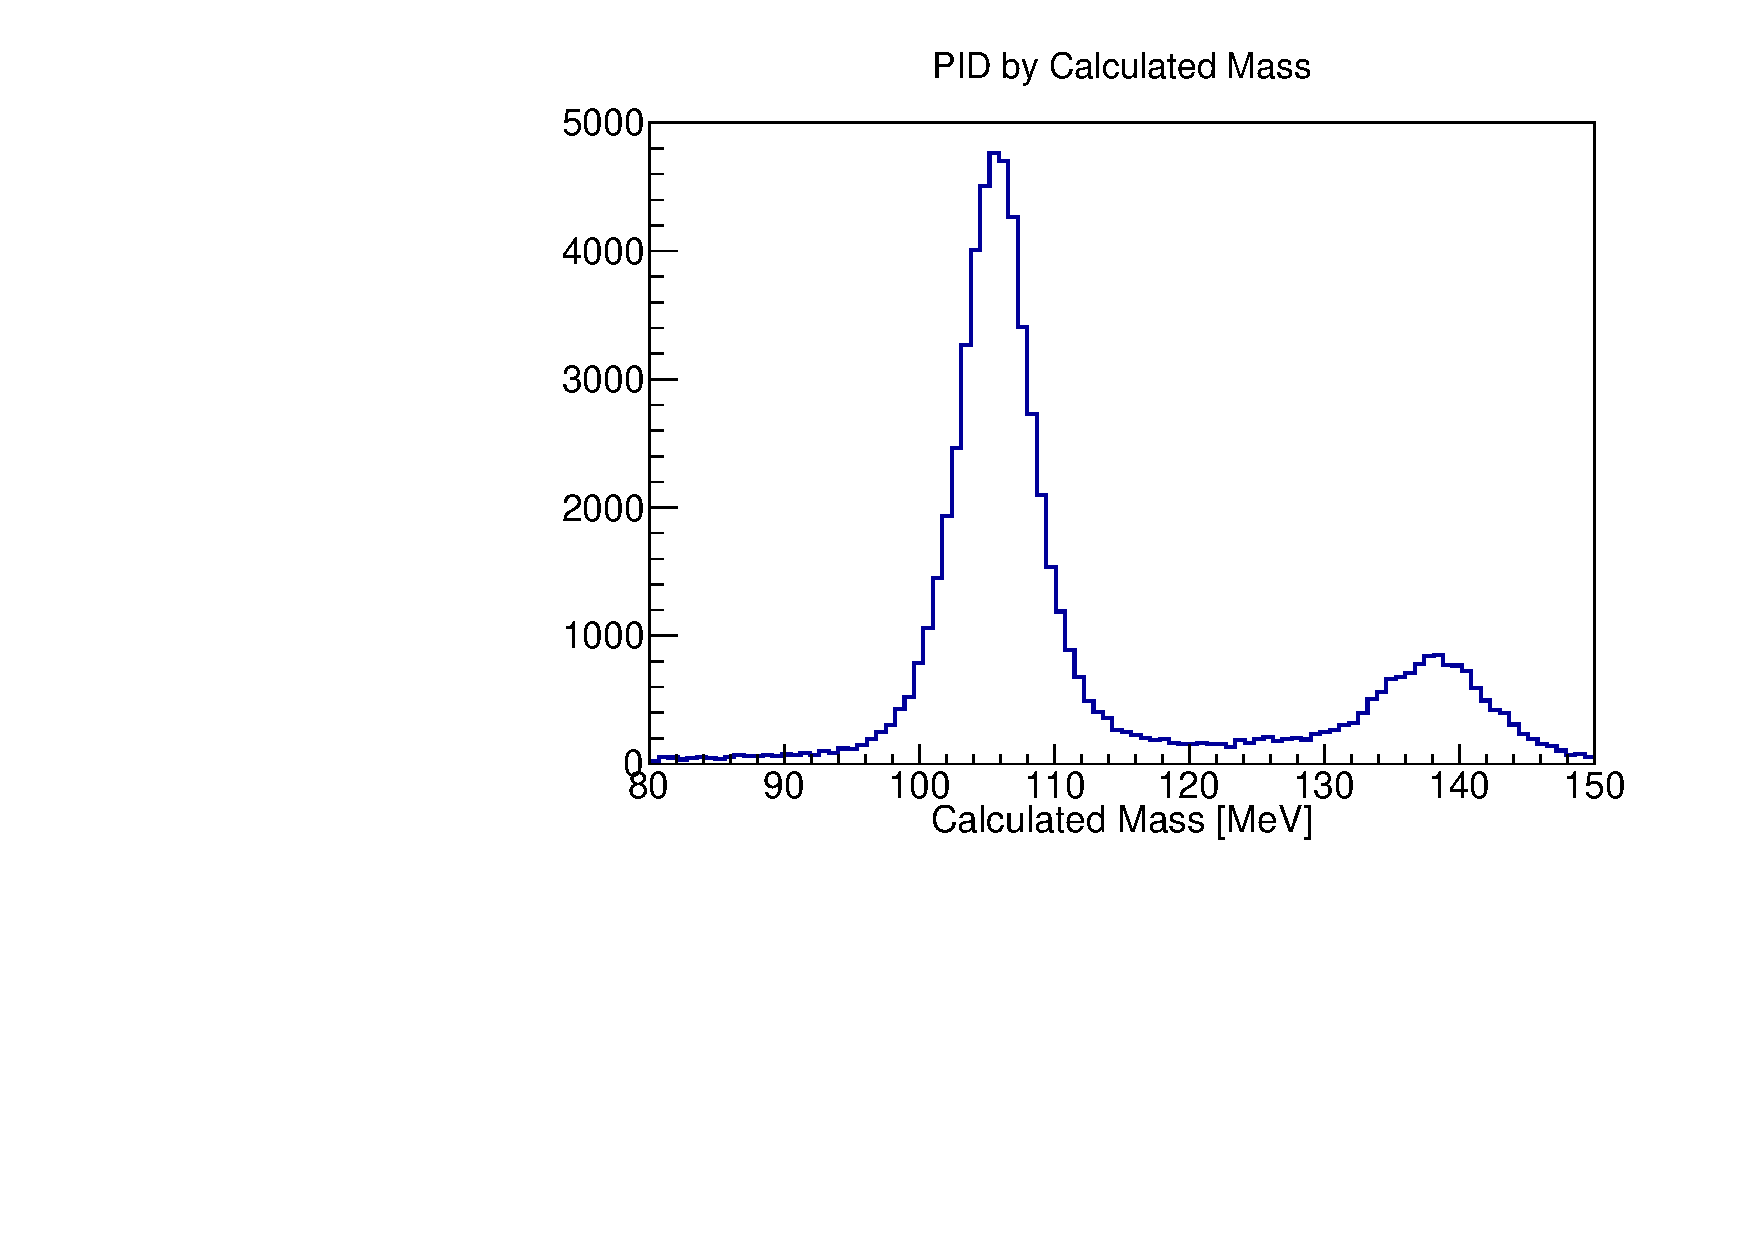
\includegraphics[width=0.45\textwidth]{calc_mass.pdf}}
\caption{The calculated mass of particles using the PID algorithm.}
\label{fig:pid_mass}
\end{figure}


\subsection{Performance of the PID}
\label{SubSect:PID_Performance}
{\color{red}
\begin{itemize}
\item add efficiency/purity curve
\item compare US/DS measurements
\end{itemize}
}


\begin{comment}
Intro:
	
Algo:
	TOF/Tracker
	EMR/Tracker?
Performance:
	comparison of US and DS, calculate additional pi -> mu decays?
	figure comparing US mass and DS mass?
\end{comment}


\begin{comment}
proton_absorber
Proton Contamination Studies in the MICE Muon Beam Line
S. Blot, Y.K. Kim (Chicago U.), R.R. Fletcher (UC, Riverside), D. Kaplan (IIT, Chicago), C. Rogers (Rutherford). Sep 2011. 3 pp.
IPAC-2011-MOPZ034 

pion_contamination
???

\end{comment}
